% CoRL 2026 Workshop "Do Robots Need World Models? A Debate on Dynamics Learning, Planning, and
% End-to-End Robot Learning" (https://do-robots-need-world-models.github.io) -- DRAFT v1 (2026-10-03)
% Research-paper track. Up to 4 pages, CoRL template. Submit on OpenReview:
% https://openreview.net/group?id=robot-learning.org/CoRL/2026/Workshop/do-robots-need-world-models
% Deadline 2026-10-12; notification 10-26; camera-ready 11-06; workshop 11-12. Reciprocal review: one
% author must review another submission. Archival: TBD. Not double-blind as far as the page says;
% kept anonymous to be safe. References assumed outside the 4 pages (CoRL convention): check.
% Build: cd paper && tectonic -X compile main.tex  (corl_2026.sty, corlabbrvnat.bst: official kit).
\documentclass{article}
\usepackage{corl_2026}             % official CoRL 2026 submission style (anonymous); [final] for camera-ready
\usepackage[T1]{fontenc}           % Times (ptm) under XeTeX/Tectonic; harmless under pdfLaTeX
\usepackage{booktabs,amsmath,amssymb,graphicx,xcolor}
\newcommand{\todo}[1]{\textcolor{red}{[TODO: #1]}}

\title{Accurate on Average, Blind at the Fork}
\author{Anonymous Authors}

\begin{document}
\maketitle

\begin{abstract}
Some safety questions are counterfactual: would a slightly different execution of this action, or a
slightly different version of the perceived scene, end in a different regime? Following the human
intuitive physics engine \citep{battaglia2013simulation}, we answer them with a goal-free
\emph{fork probe} that samples the robot's measured execution and perception error, rolls out 64
futures, and alarms when they split into persistent, well-separated groups, with no task labels,
failure data or fitted thresholds. In simulated Jenga extraction with real camera perception, the
probe tracks ground-truth fragility on three fresh panels ($\kappa$ 0.70--0.84 against a ceiling of
0.85--0.92, versus 0.32--0.51 when perception error is ignored), including when outcomes are read
from image tokens. Used to evaluate a world model, the probe exposes a failure that average error hides: a stochastic
token-space world model that predicts futures well on average reaches only $\kappa$ 0.18, because its
sampled spread is isotropic and ignores where futures branch. Robots need world models for such questions, but only ones with this \emph{branching
fidelity}, which current models lack and current benchmarks do not measure.
\end{abstract}

\keywords{World models, intuitive physics, runtime safety}

\section{Introduction}
Modern manipulation policies, from diffusion policies to vision-language-action models, act by
committing to short \emph{action chunks} \citep{chi2023diffusion,zhao2023act,black2024pi0}. Before a
chunk runs, a safety monitor can ask whether it is safe. In contact-rich tasks such as Jenga
extraction the answer hinges on millimetres: the same command can slide the block out or tip a
neighbour, depending on small errors in execution and perception. Such a chunk is precarious even if
its nominal rollout succeeds, because uncertainty the robot cannot control decides the outcome.

People judge precariousness in a similar way. In the \emph{intuitive physics engine} (IPE) account
\citep{battaglia2013simulation}, observers run a few approximate, noisy simulations over an uncertain
scene and call it unstable when the simulated outcomes disagree; noise in both perception and dynamics
is needed to explain human judgments \citep{smith2013sources,sanborn2013reconciling}. We give a robot
the same recipe: perturb the chunk with its \emph{measured} execution error and the scene with its
\emph{measured} perception error, roll out 64 futures, and flag the chunk when they split into
distinct outcomes. This needs a model the robot can query, and makes the world-model debate concrete:
such a model helps only if its rollouts branch where the real dynamics branch.

\paragraph{Contributions.} (1) A \emph{fork probe} that validates an action chunk before execution
without task labels, failure data or fitted thresholds (Sec.~\ref{sec:method}). (2) Evidence, with a
real camera-based perception model on three fresh test panels, that sampling the robot's own
perception error is what makes the judgment match ground truth, including when outcomes are read
directly from image tokens (Sec.~\ref{sec:perception}). (3) \emph{Branching fidelity} as a world-model
evaluation: a token-space world model that predicts well on average still loses the forks, and a
diagnosis shows where its uncertainty should live instead (Sec.~\ref{sec:wm}).

\section{Problem setup and fork probe}\label{sec:method}
\paragraph{Task and monitor.} A simulated Franka Panda (MuJoCo) extracts blocks from Jenga-like
stacks. At every chunk start a policy commits to an 8-step action chunk, held for 30 further steps.
In our experiments the chunks come from recorded extraction episodes, but the monitor treats the
policy as a black box: it sees only the commanded chunk, one camera image and the robot's
proprioception, so it applies unchanged to any chunked policy. (How it rolls out futures, with a
simulator or a learned model, is the subject of Sec.~\ref{sec:wm}.)

\paragraph{What we call unsafe.} A chunk is \emph{fragile} if deviations the robot cannot control,
namely its execution error and the error in its perception of the scene, can send the outcome into
qualitatively different regimes. Three reasons motivate this definition. It is \emph{task- and
policy-agnostic}: it needs no goal predicate or failure label, which a monitor around a generalist
policy cannot assume. It isolates cases where the robot's \emph{intent no longer determines the
outcome}; if all plausible executions agree, the result is a property of the plan. And in contact-rich
manipulation damage typically happens at such boundaries, which we verify against physical harm. A
chunk that fails \emph{deterministically} is not flagged; that needs a task-level check.

\paragraph{Fork probe.} We draw 64 execution-error snippets from the robot's measured tracking
residuals (median chunk maximum 3.2\,mm), subtract them from the commanded positions, and roll out.
The probe alarms if, at hold steps 10 \emph{and} 30, the endings (object positions, or later image
tokens) projected on their first principal axis prefer two Gaussians to one by BIC, are well
separated (Ashman's $D>2$ \citep{ashman1994detecting}), have at least 2 rollouts in the minority, and
keep the same partition. These constants are fixed statistical conventions, not fitted to labels.

\paragraph{Uncertainty-aware probes.} The robot does not see the true scene $s$ but an estimate
$\hat s$: a frozen DINOv2 encoder \citep{oquab2024dinov2} on one close-camera image plus a keypoint
head regresses the poses of the three blocks in play (held-out error 2.5\,mm). Its validation
residuals define an error model (full $9\times9$ position covariance plus rotation covariances). The
\emph{naive} probe starts every rollout at $\hat s$. The \emph{aware} probe (v1) starts rollout $j$ at
$\hat s+e_j$, with $e_j$ drawn from the error model, as the IPE does. The \emph{Bayesian} probe (v2)
draws 5 hypotheses $\hat s+d_m$, runs an aware probe around each, and alarms if at least 3 split.

\paragraph{Ground truth and protocol.} \emph{Fragility truth} applies the aware recipe around the
\emph{true} state with exact physics, so it reflects the robot's uncertainty, not one exact outcome. Two independent seeds (A, B) agree at Cohen's $\kappa$ 0.85--0.92, the attainable
ceiling. Because this truth shares the split test with the monitors, it measures how well a monitor
handles perception, not whether splits are dangerous. For that we use an independent physical label:
a \emph{harm fork} is a state where 2--62 of 64 truth rollouts topple a neighbouring block. Every
confirmation uses a \emph{fresh panel} of unseen stack layouts (up to 60 topple forks plus 100 safe
states) under a protocol frozen before the data existed.

\section{Results}
With exact physics and the true state, the split test alarms on all 23 development topple forks at a
10\% alarm rate on quiet states. What remains when the robot relies on its own perception, and then on
a learned model instead of the simulator?

\begin{figure}[t]
\centering
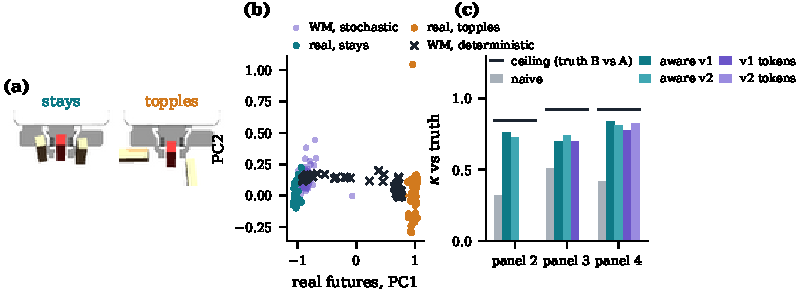
\includegraphics[width=\linewidth]{fig_forks.pdf}
\caption{(a) Two of 64 endings of one panel-3 chunk under execution error: the neighbour stays or
topples. (b) A held-out fork: real latent futures (colour = outcome) on their principal axes, with the
token world models' futures for the same inputs; the deterministic model spreads along the branch axis,
the stochastic one stays near one outcome. (c) Agreement with fragility truth on three fresh panels; lines mark the ceiling.}
\label{fig:forks}
\end{figure}

\subsection{Handling perception error}\label{sec:perception}
Real perception errors of 2--4\,mm are comparable to execution noise, so the perceived scene is
effectively a different scene. The naive probe, which trusts $\hat s$, reaches only 38--55\% of the
ceiling $\kappa$; sampling the measured perception error raises this to 76--91\%
(Table~\ref{tab:panels}, Fig.~\ref{fig:forks}c), and the aware probes catch 77--91\% of harm forks.
This is the IPE's prescription: judge fragility at one's own uncertainty, not at a point estimate.

\begin{table}[t]
\centering
\caption{Fork probes with real perception on fresh panels (exact physics). $\kappa$: agreement with
fragility truth A; harm: recall on harm forks; tokens: outcomes read from image tokens.}
\label{tab:panels}
\small
\begin{tabular}{lcccccc}
\toprule
& \multicolumn{2}{c}{Panel 2 (153 states)} & \multicolumn{2}{c}{Panel 3 (160)} & \multicolumn{2}{c}{Panel 4 (156)} \\
monitor & $\kappa$ & harm & $\kappa$ & harm & $\kappa$ & harm \\
\midrule
ceiling (truth B vs A) & 0.85 & -- & 0.92 & -- & 0.92 & -- \\
naive ($\hat s$ only) & 0.32 & -- & 0.51 & 0.65 & 0.42 & 0.67 \\
aware v1 & 0.76 & -- & 0.70 & 0.77 & 0.84 & 0.91 \\
aware v2 (Bayesian) & 0.73 & 0.90 & 0.74 & 0.90 & 0.82 & 0.89 \\
aware v1, tokens & -- & -- & 0.70 & 0.77 & 0.77 & 0.88 \\
aware v2, tokens & -- & -- & -- & -- & \textbf{0.83} & \textbf{0.88} \\
\bottomrule
\end{tabular}
\end{table}

\paragraph{Reading outcomes from images.} A deployed monitor should not need object states to judge
outcomes either. Applied unchanged to DINOv2 tokens of rendered endings, the split test gives almost
the same decisions ($\kappa$ 0.86--0.90 with the position-based test), and the fully visual Bayesian
probe meets its frozen harm gate on panel 4 (recall 0.88, 95\% CI 0.77--0.94; 7\% alarms on non-harm
states). Remaining misses come from where rollouts start, not from reading images: on panel 3, 12 of
14 missed harm forks arose because the single estimate put the whole rollout cloud on the safe side of
the edge.

\subsection{Branching fidelity of learned world models}\label{sec:wm}
So far, rollouts ran in MuJoCo with the true geometry; only the block poses came from the camera.
Outside simulation a learned model must take that role, and the fork probe becomes its test: given one
image and the 64 perturbed chunks, do its rollouts branch where physics branches? Our candidate encodes the image with DINOv2,
compressed by a fixed per-patch PCA to a $28\times28\times8$ latent (chosen beforehand to keep pose
and fork information). A flow-matching transition predicts
the next latent from the current one and the action, with fresh noise at every step, so that repeated
rollouts can differ. It is trained on 8 futures per image whose start scenes were sampled within the
measured perception error, so the spread of its targets is exactly the robot's own uncertainty. A
deterministic version with the same architecture serves as control. Both predict well on average:
they beat a no-motion baseline on 19-step latent error by 3--4$\times$. Yet the stochastic model fails
on fresh panel 4 ($\kappa$ 0.18, harm recall 0.18; Table~\ref{tab:wm}), below its deterministic
control ($\kappa$ 0.42).

\begin{table}[t]
\centering
\caption{Token world models: panel 4 ($\kappa$, harm) and diagnostics on 60 held-out states.}
\label{tab:wm}
\small
\begin{tabular}{lccccc}
\toprule
dynamics & $\kappa$ & harm & spread & PC1 & ratio \\
\midrule
reference (MuJoCo + v2 tokens; real futures) & 0.83 & 0.88 & 1.00 & 0.57 & 4.8 \\
token WM, stochastic & 0.18 & 0.18 & 0.98 & 0.15 & 1.3 \\
token WM, deterministic & 0.42 & 0.60 & 0.04 & 0.69 & 32 \\
\todo{iteration 2} & & & & & \\
\bottomrule
\end{tabular}
\end{table}

\paragraph{Why the stochastic model fails.} Table~\ref{tab:wm} compares total spread, its share on the
main axis (PC1) and its fork/non-fork ratio with real futures. The model reproduces the \emph{amount} of spread but not its
\emph{shape} or \emph{placement}: the spread is isotropic and nearly equal on forks and non-forks, the
average uncertainty of futures rather than where they branch; other samplers are worse. The deterministic model's spread is tiny but aligned
with the branch axis and 32$\times$ larger on forks (Fig.~\ref{fig:forks}b); started from rendered
perturbed scenes it doubles agreement with real futures ($\kappa$ 0.17$\to$0.37). Per-step noise is not wrong in general
(diffusion weather ensembles stay well dispersed \citep{price2025gencast}); ours was misplaced. Here, as in the IPE, the uncertainty that
matters is in the initial conditions, and roughly right dynamics amplify it along the branch. A second iteration (a learned operator perturbing the start
latent by physical perception error, then deterministic dynamics) is under evaluation \todo{result}.

\section{Related work}
\paragraph{Simulation under uncertainty.} Beyond the IPE and counterfactual accounts of physical
support \citep{zhou2023mental}, robotics runs Monte Carlo rollouts over pose, friction or model
parameters to score grasps and pushes \citep{mahler2017dexnet,agboh2018pushing} or to build safety
filters \citep{johansson2025safety,wang2026manidreams}. Closest to our setup, \citet{cannizzaro2024cobra}
sample measured perception and placement noise through a simulator to predict whether a block tower
stands, and \citet{goyal2026stability} perturbs action chunks with policy-scale noise to measure, offline,
how fast deviations grow. These score a task predicate, labels \citep{lerer2016learning} or a growth rate;
\citet{zapolsky2016particle} proposed goal-free detection of divergent particle traces but evaluated
task failure. We judge only whether the outcome set splits, a Monte Carlo test of proximity to a basin
boundary \citep{menck2013basin}.
\paragraph{Runtime monitors.} Latent safety filters use learned failure classifiers, also on Jenga
\citep{nakamura2025generalizing,seo2025uncertainty}; failure detectors use policy uncertainty calibrated
on successes \citep{xu2025failure,agia2024unpacking}. Both measure what a model does not know, not
whether the physics is at a branch.
\paragraph{World models and their uncertainty.} Learned simulators and latent world models
\citep{sanchezgonzalez2020learning,allen2023fignet,zhou2025dinowm,assran2025vjepa2,hafner2025dreamerv3}
struggle with stiff contact \citep{parmar2021fundamental}, and audits find poor physical grounding and
optimism under failure-inducing actions \citep{bear2021physion,motamed2026physicsiq,yang2026mirabench}. \citet{yu2026evaluated}
propose evaluating world models on interventional action branches by per-branch error; our models
have low error yet lose the forks. Stochastic and ensemble models
\citep{chua2018pets,lakshminarayanan2017ensembles} are judged by likelihood or return, not by where
their spread falls.

\section{Conclusion and limitations}
A robot can judge fragility the way people do, by sampling its own perception and execution
uncertainty through a rough simulator. For the question this workshop poses, our results suggest that
pre-execution safety checks of this kind need a queryable world model with branching fidelity, which
the world models we trained lack despite low average error, and that, in this setting, the uncertainty that
matters enters through the initial conditions. Average-error benchmarks would rank these models
well; branching fidelity is a needed additional axis. \paragraph{Limitations.} Simulation, one task family, three tracked blocks; MuJoCo probes use
privileged geometry beyond the perceived poses; fragility truth shares the split test (harm forks are the
independent check); panels vary; single world-model runs; deterministic failures are not flagged.

\bibliography{references}
\end{document}
